\section{Penelitian dan Riset Terkait}
\label{sec:riset-terkait}

\subsection{China Electronic Toll Colleciton}
China memiliki masyarakat yang sangat banyak dan setiap masyarakat memiliki sekurang kurangnya satu kendaraan. Seiring bertambah nya masyarakat di China, maka jalanan yang ada di China akan semakin penuh dengan kendaraan yang akan menghasilkan kemacetan terutama pada tol bagian pembayaran. Untuk mengatasi masalah ini China menggunakan \textit{Electronic Toll Colleciton (ETC)} yang di integrasikan dengan setiap kendaraan untuk mempercepat proses ini \parencite{penelitianterkait1}.

China menggunakan KubeEdge untuk melakukan proses \textit{deployment} \textit{ETC} untuk 100,000 \textit{nodes} dengan total 500,000 aplikasi yang diluncurkan menggunakan KubeEdge tersebar untuk 29 dari 34 provinsi. Proses \textit{deployment} dilakukan secara otomatis dengan membuat sistem \textit{workflow engine} pada kubernetes sehingga proses \textit{deployment} dapat dilakukan dengan cepat dan mudah. Dengan menggunakan metode ini sistem pembayaran tol di China menjadi 10x lebih cepat dari sebelumnya \parencite{penelitianterkait1}.


\begin{figure}[h]
  \centering
  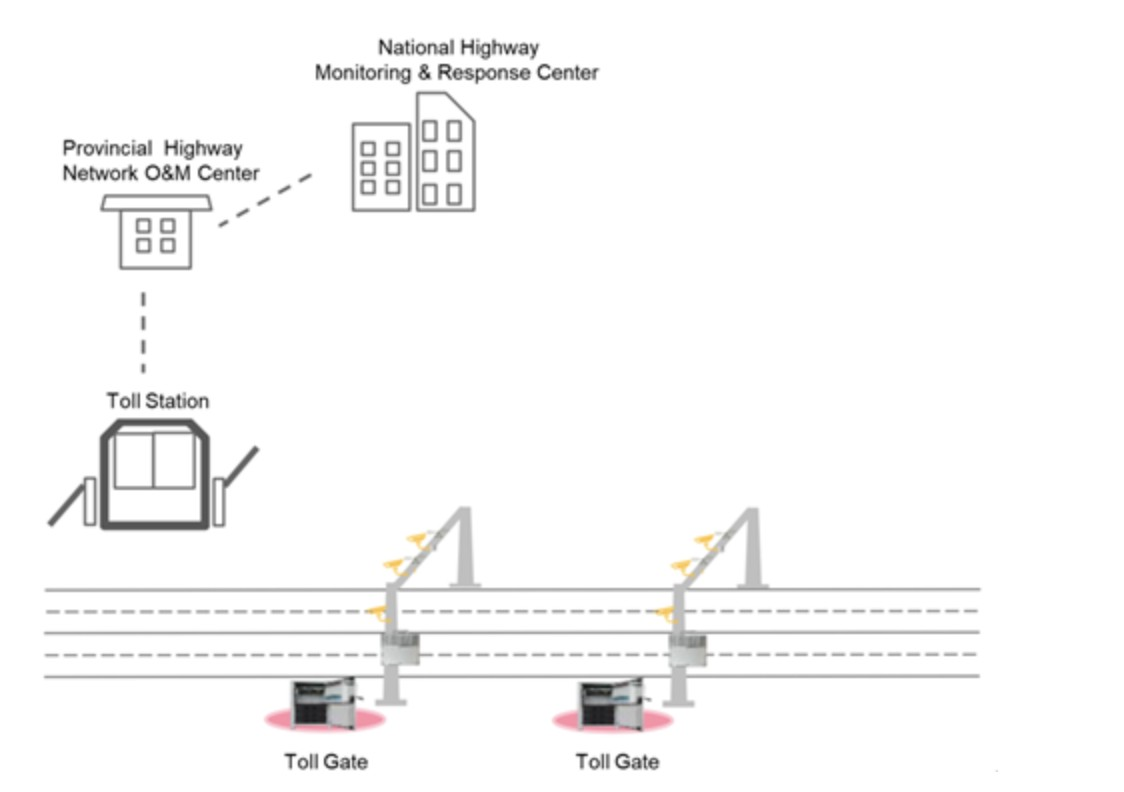
\includegraphics[width=0.8\textwidth]{resources/chapter-2/china-highways.jpg}
  \caption{Implementasi sistem \textit{ETC} di China \parencite{penelitianterkait1}}
  \label{fig:china-highways}
\end{figure}

\begin{figure}[h]
  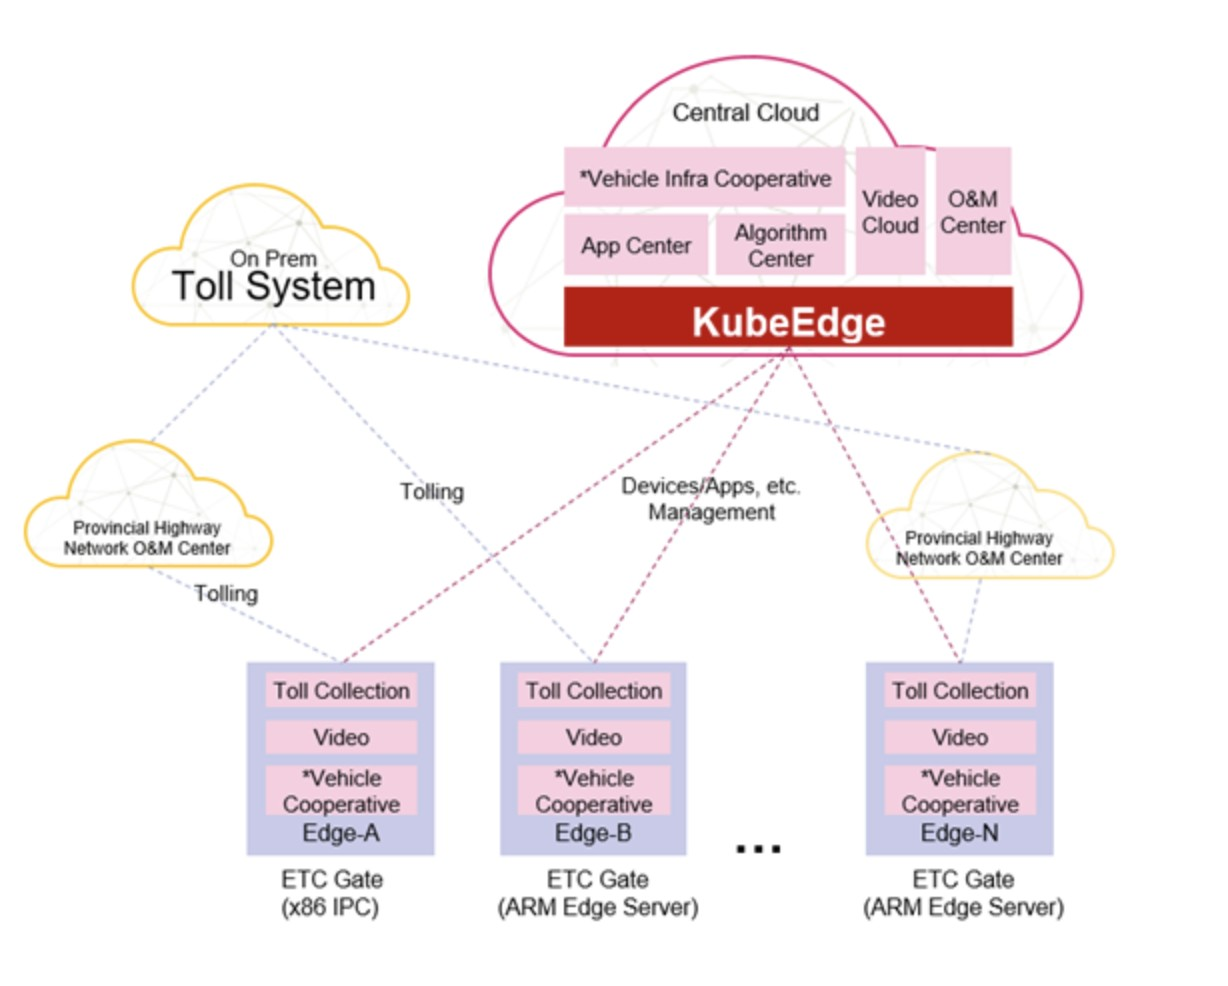
\includegraphics[width=0.8\textwidth]{resources/chapter-2/arsitektur-china-highways.jpg}
  \caption{Arsitektur sistem \textit{ETC} di China \parencite{penelitianterkait1}}
  \label{fig:architecture-china-highways}
\end{figure}

\subsection{A Model for the Remote Deployment, Update, and Safe Recovery for Commercial Sensor-Based IoT Systems}
Penelitian ini menggali tantangan-tantangan khusus terkait infrastruktur yang didedikasikan untuk penyebaran dan manajemen aplikasi secara jarak jauh, membahas tantangan-tantangan manajemen terkait sistem sensor IoT, dan mengusulkan sebuah model matematis serta metodologi untuk mengatasi hal tersebut. Untuk menguji efisiensi model ini, kami mengimplementasikannya sebagai sistem infrastruktur perangkat lunak untuk produk IoT bisnis yang lengkap. Sebagai bukti, kami menyajikan penyebaran 100 mesin penjual minuman smart di tiga lokasi. Setiap mesin bergantung pada sensor yang memantau statusnya dan pada gateway yang mengendalikan perilakunya, menerima 133 pembaruan perangkat lunak jarak jauh yang berbeda melalui solusi kami. Selain itu, 80\% mesin beroperasi tanpa gangguan selama 250 hari, dengan 20\% mengalami kegagalan akibat faktor eksternal; dari 80\% tersebut, 30\% mengalami kegagalan pembaruan sementara akibat kapabilitas perangkat keras yang berkurang dan sistem dengan berhasil melakukan pemulihan otomatis dalam 100\% kegagalan sementara tersebut \parencite{RemoteDeployment}.

\begin{figure}[h]
  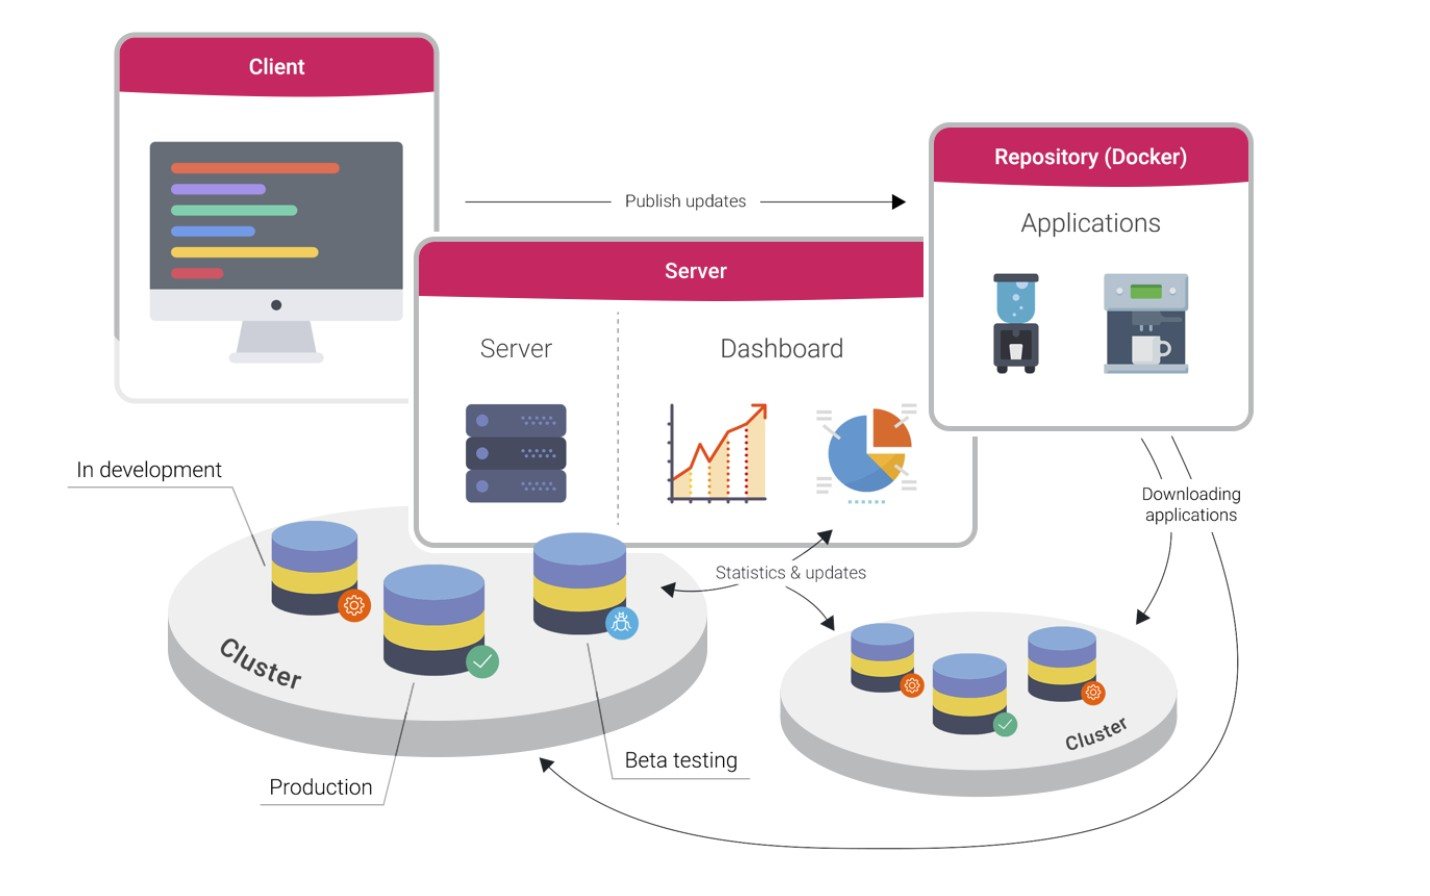
\includegraphics[width=0.8\textwidth]{resources/chapter-2/arsitektur-remote-deployment.jpg}
  \caption{Arsitektur remote \textit{deployment} \parencite{RemoteDeployment}}
  \label{fig:architecture-remote-deployments}
\end{figure}


\subsection{Device discovery strategies for the IoT}
Penelitian ini membahas mengenai beberapa strategi untuk melakukan deployment pada IoT. Pada penelitian ini menyebutkan bahwa terdapat tiga jenis deployment yang dilakukan oleh

\parencite{DeviceDiscovery}


